\documentclass[tikz,border=4pt]{standalone}
\usepackage[T1]{fontenc}
\usepackage{lmodern}
\renewcommand{\familydefault}{\sfdefault}
\usetikzlibrary{shapes.geometric,positioning,arrows.meta,calc}
\tikzset{
  node distance=6mm,
  every node/.style={font=\footnotesize,align=center,execute at begin node={\hyphenpenalty=10000\relax}},
  base/.style={draw=gray!60,fill=gray!12,minimum height=7mm,inner sep=2pt},
  term/.style={base,rounded corners=3.5mm,text width=30mm},
  proc/.style={base,text width=32mm},
  err/.style={base,text width=30mm,fill=gray!22},
  io/.style={base,trapezium,trapezium left angle=72,trapezium right angle=108,trapezium stretches=true,text width=28mm},
  dec/.style={base,diamond,aspect=2.4,text width=27mm,inner sep=0pt},
  go/.style={-{Stealth[length=2mm]},draw=gray!55!black},
  lab/.style={font=\scriptsize,fill=white,inner sep=1pt},
}

\begin{document}
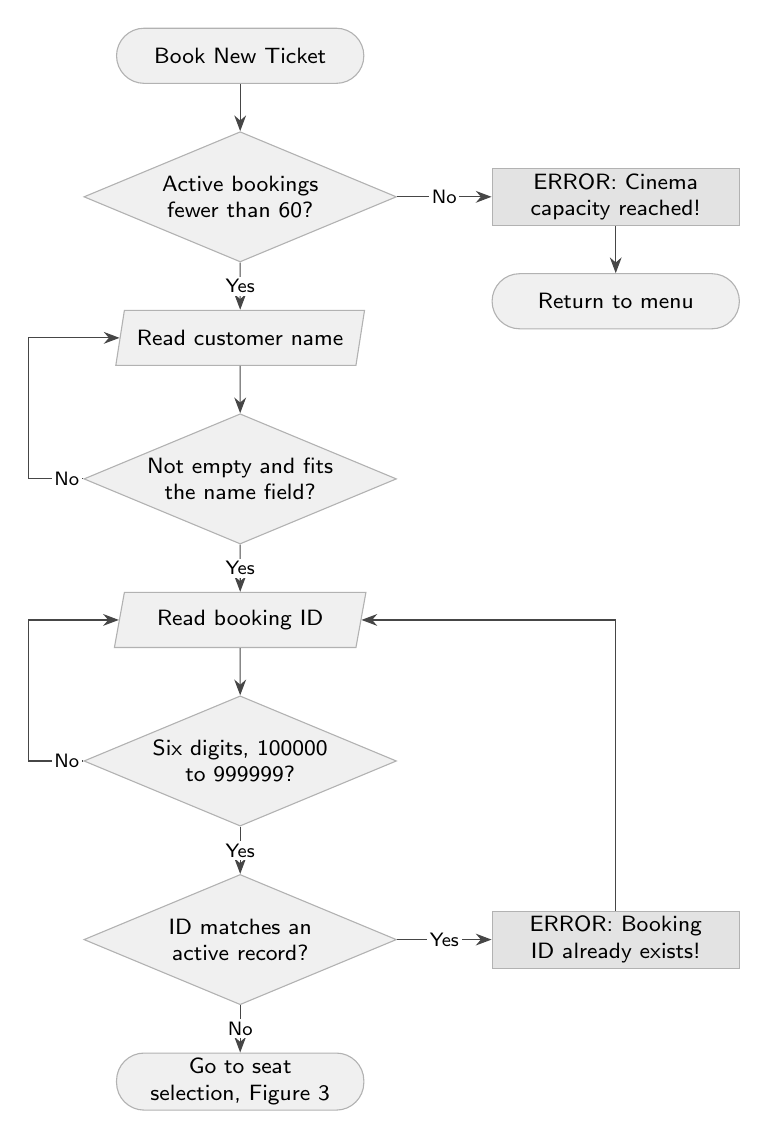
\begin{tikzpicture}
\node[term] (s) {Book New Ticket};
\node[dec,below=of s] (d1) {Active bookings fewer than 60?};
\node[err,right=12mm of d1] (e1) {ERROR: Cinema capacity reached!};
\node[term,below=of e1] (r1) {Return to menu};
\node[io,below=of d1] (n) {Read customer name};
\node[dec,below=of n] (d2) {Not empty and fits the name field?};
\node[io,below=of d2] (i) {Read booking ID};
\node[dec,below=of i] (d3) {Six digits, 100000 to 999999?};
\node[dec,below=of d3] (d4) {ID matches an active record?};
\node[err,right=12mm of d4] (e2) {ERROR: Booking ID already exists!};
\node[term,below=of d4] (g) {Go to seat selection, Figure 3};
\draw[go] (s)--(d1);
\draw[go] (d1)--node[lab]{Yes}(n);
\draw[go] (d1)--node[lab]{No}(e1);
\draw[go] (e1)--(r1);
\draw[go] (n)--(d2);
\draw[go] (d2)--node[lab]{Yes}(i);
\draw[go] (d2.west)--node[lab,pos=.3]{No}++(-7mm,0)|-(n.west);
\draw[go] (i)--(d3);
\draw[go] (d3)--node[lab]{Yes}(d4);
\draw[go] (d3.west)--node[lab,pos=.3]{No}++(-7mm,0)|-(i.west);
\draw[go] (d4)--node[lab]{No}(g);
\draw[go] (d4)--node[lab]{Yes}(e2);
\draw[go] (e2.north)|-(i.east);
\end{tikzpicture}
\end{document}
